\chapter{Analisis Persoalan dan Rancangan Solusi}

Tujuan utama penulisan bab ini adalah untuk menguraikan rencana penyelesaian masalah ::TODO: fill::. Bagian ini memaparkan proses analisis masalah hingga menjadi solusi.


\section{Analisis}

\section{Analisis Permasalahan}
\label{sec:analisis-permasalahan}

% Berdasarkan latar belakang yang telah diuraikan pada \ref{sec:latar-belakang}, penggunaan \textit{erasure coding} pada sebuah sistem dapat mengurangi kebutuhan penyimpanan data dengan tetap menjaga integritas dan ketahanan data. Walaupun membutuhkan sumber daya komputasi dalam penerapannya, pengurangan ukuran data keseluruhan yang diperlukan menyebabkan juga turunnya ukuran data yang perlu dikirim ke \textit{node} lainnya.Hal ini menyebabkan mungkinnya terdapat suatu kondisi ketika {response time} yang diperlukan untuk melakukan operasi pada \textit{erasure coding} lebih rendah jika dibandingkan dengan melakukan operasi yang sama pada sistem yang menggunakan \textit{replikasi} untuk mencapai ketahanan tersebut.

Berdasarkan latar belakang dan studi literatur yang telah ditentukan, \textit{erasure coding} memiliki potensi untuk menghasilkan \textit{response time} yang lebih rendah dibandingkan dengan sistem berbasis \textit{replikasi} karena walaupun membutuhkan komputasi, ukuran data yang dikirimkan untuk ketahanan lebih rendah dibandingkan replikasi. Riset ini akan menganalisis faktor-faktor untuk mencapai kondisi tersebut. Faktor yang dianalisis antara lain ukuran data yang besar dan jaringan yang lambat. Dengan demikian, diperlukan sistem yang dapat mensimulasikan operasi pada sistem \textit{erasure coding} dan replikasi sekaligus memvariasikan faktor-faktor tersebut dalam operasinya tanpa memengaruhi kinerja sistem di sisi lain.

Dari permasalahan tersebut, dirumuskan kebutuhan sebuah perangkat lunak antara lain
\begin{enumerate}

    \item Sistem harus dapat mensimulasikan kondisi \textit{database} terdistribusi yang menggunakan replikasi ataupun \textit{erasure coding}.
    \item Sistem harus dapat menyimpan data secara \textit{persistent}.
    \item Sistem harus dapat memvariasikan ukuran data dan kecepatan jaringan.
    \item Sistem harus dapat menjalankan eksperimen berulang kali untuk mendapatkan data dari eksperimen.

\end{enumerate}

Penjelasan lebih detail mengenai kebutuhan sistem terdapat pada lampiran \ref{sec:rancangan-struktural}.

\subsection{Alternatif Solusi}
\label{sec:analisis-solusi}

Berdasarkan analisis permasalahan pada bagian \ref{sec:analisis-permasalahan} serta studi literatur, Terdapat tiga alternatif solusi dalam pembuatan PERISAI. yaitu membuat arsitektur berbasis Kubernetes, arsitektur berbasis \textit{apache zookeper}, serta membuat arsitektur dengan mengikuti referensi yang sudah ada.

\subsubsection{Membuat sistem berbasis Kubernetes}
Kubernetes, sebagai layanan orkestrasi kontainer yang kuat, menawarkan mekanisme otomatisasi \textit{deployment}, skalabilitas, dan manajemen aplikasi yang sangat cocok untuk lingkungan \textit{cloud} dan terdistribusi. Dalam konteks IoT, Kubernetes bisa dimanfaatkan untuk mengelola dan mengorkestrasi aplikasi berbasis kontainer pada lingkungan IoT ataupun pada \textit{cloud}. Kubernetes mendukung model \textit{microservices} yang fleksibel dan resilien serta memiliki banyak kelebihan yaitu meliputi kemampuan autoscaling, pemulihan otomatis dari kegagalan, dan manajemen beban kerja yang efisien. Kubernetes dapat memanfaatkan \textit{affinity selector} untuk melakukan \textit{targeted deployment}, sehingga proses \textit{deployment} dapat diberikan kepada perangkat yang memerlukan \textit{deployment} saja. Namun, Kubernetes juga memiliki kekurangan yaitu membutuhkan sumber daya yang relatif tinggi, yang mungkin tidak ideal untuk perangkat IoT dengan keterbatasan sumber daya. Namun, hal ini dapat diatasi dengan distribusi Kubernetes yang khusus dibuat untuk lingkungan IoT yaitu microk8s, K3s, serta KubeEdge. Dari ketiga solusi ini, distribusi K3s dapat dijalankan pada perangkat yang hanya memiliki RAM 900mb tanpa ada masalah. Selain itu kemudahan dalam penggunaan dan supportnya untuk seluruh arsitektur membuat K3s menjadi pilihan yang digunakan untuk tugas akhir ini. Perbandingan ketiga distribusi dapat dilihat pada lampiran \ref{tab:perbandingan-distribusi-kubernetes}.

\subsubsection{Membuat sistem berbasis \textit{Apache ZooKeper}}
Apache ZooKeeper menyediakan layanan koordinasi terdistribusi yang sangat diperlukan pada lingkungan aplikasi terdistribusi. Dalam konteks sistem \textit{remote deployment} pada lingkungan IoT, ZooKeeper dapat dimanfaatkan untuk mengelola konfigurasi dan melakukan sinkronisasi diantara komponen sistem terutama pada lingkungan terdistribusi. Kelebihan menggunakan ZooKeeper antara lain konsistensi data yang tinggi dan model pemrograman yang relatif sederhana. Kekurangannya, ZooKeeper tidak secara langsung mendukung kasus \textit{deployment} aplikasi karena hanya berfokus pada masalah konfigurasi, Selain itu zookeper juga membutuhkan \textit{resource} yang sangat besar sehingga bisa menjadi \textit{bottleneck} jika tidak dirancang dengan hati-hati, terutama dalam lingkungan dengan jumlah perangkat yang sangat besar. Zookeper juga tidak Oleh karena itu, diperlukan adanya penyesuaian dan adopsi agar menjadi kompatibel dan tidak menjadi \textit{bottleneck}.

\subsubsection{Membuat sistem berbasis LEONORE dan DIANE}
Mengembangkan sistem provisioning skala besar berbasis LEONORE dan DIANE sudah menyelesaikan beberapa masalah yang telah disebutkan. Namun kekurangannya ialah, desain menjadi tidak fleksibel, sulit untuk dikustomisasi, serta terdapat resiko keamanan jika tidak mengimplementasikan dengan benar. Selain itu proses implementasi membutuhkan waktu yang lama. Proses pengujian yang sulit pun menjadi salah satu tantangan dalam mengimplementasikan metode ini.

\pagebreak

Berdasarkan ketiga alternatif solusi yang telah dijelaskan, Dipilihlah kubernetes sebagai dasar dari PERISAI. Alasan pemilihan kubernetes karena menjawab permasalahan yang telah dijelaskan pada bagian \ref{sec:analisis-permasalahan} khususnya \textit{targeted deployment}.Perbandingan ketiga alternatif solusi dapat dilihat pada tabel \ref{tab:perbandingan-analisis-solusi}.

\bgroup
\begin{table}[ht]
  \def\arraystretch{1.3}
  \caption{Perbandingan Ketiga Alternatif Solusi}
  \label{tab:perbandingan-analisis-solusi}
  \centering
  \begin{tabular}{|p{2cm}|p{2cm}|p{2cm}|p{1.8cm}|p{1.7cm}|p{1.7cm}|}
    \hline
    Solusi           & Berjalan di berbagai perangkat                            & Melakukan \textit{targeted deployment} & Berjalan pada perangkat dengan sumber daya terbatas & Mengatur banyak perangkat & Waktu pembuatan sistem \\
    \hline
    Kubernetes       & Ya, seluruh perangkat yang dapat melakukan kontainerisasi & Ya                                     & Ya dengan K3s                                       & Ya                        & Cepat                  \\
    \hline
    Zookeper         & Ya, seluruh perangkat yang memiliki java                  & Tidak                                  & Tidak                                               & Ya                        & Cepat                  \\
    \hline
    LEONORE \& DIANE & Tidak                                                     & Tidak                                  & Mungkin                                             & Ya                        & Lama                   \\
    \hline
  \end{tabular}
\end{table}
\egroup

\subsection{Analisis Kebutuhan Sistem}
\label{sec:analisis-kebutuhan-sistem}

Berdasarkan bagian \ref{sec:analisis-solusi}, ::TODO: fill::.


\section{Rancangan}

\subsection{Arsitektur Sistem}
\label{subsection:system-architecture}

\begin{figure}[ht]
    \centering
    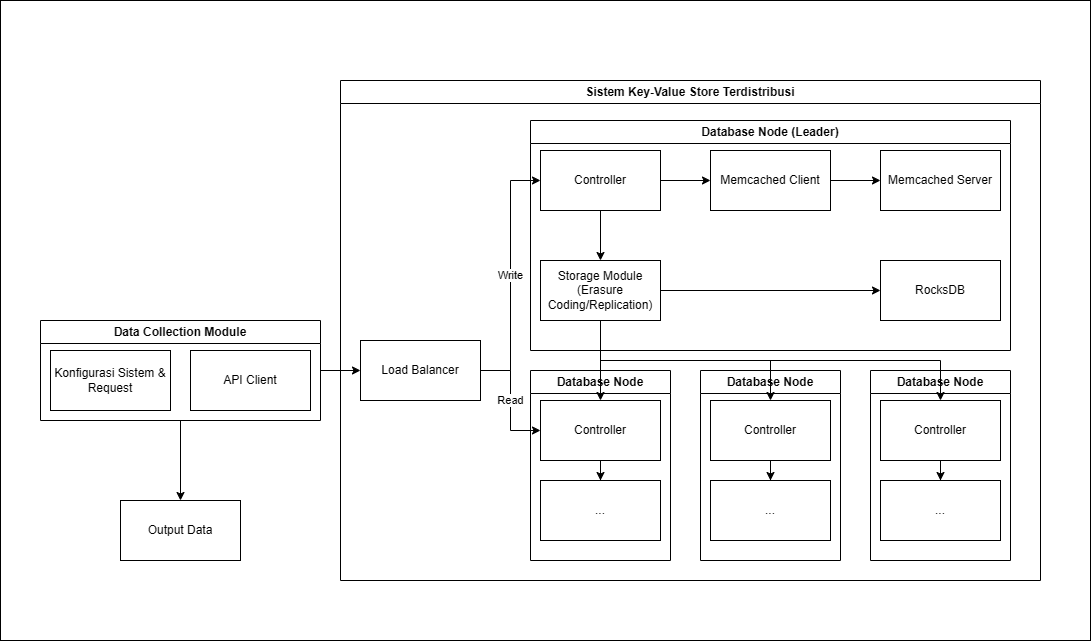
\includegraphics[width=0.95\textwidth]{resources/chapter-3/general-architecture.png}
    \caption{Gambaran Arsitektur Sistem Eksperimen}
    \label{fig:general-architecture}
\end{figure}

Arsitektur dari sistem mengasumsikan kebutuhan untuk konsistensi yang tinggi. Untuk mencapai konsistensi tersebut, operasi \textit{write} dilakukan secara \textit{synchronous} dengan distribusi replikasi dan \textit{erasure coding} dianggap selesai ketika nilai ketahanan yang diinginkan sudah tercapai.

Karena sistem bersifat terdistribusi, maka diperlukan sebuah algoritma konsensus untuk mengelola konsistensi antar \textit{Node}. Algoritma konsensus yang digunakan algoritma konsensus \textit{paxos} yang disesuaikan dengan kebutuhan. Salah satu penyesuaian yang dilakukan adalah mengadopsi pola \textit{leader-follower} untuk memudahkan sinkronisasi data dan mempercepat transaksi. Dengan adanya leader, fase 1 dari algoritma \textit{paxos} dapat dihilangkan dengan membuat proposal dari leader selalu memiliki nilai paling tinggi. Detail implementasi \textit{paxos} akan dijelaskan di bagian \ref{subsection:detail-komponen}. Diagram gambaran arsitektur sistem dapat dilihat pada gambar \ref{fig:general-architecture}.

Operasi \textit{write} akan secara ekslusif disalurkan pada \textit{leader}. Kemudian untuk ketahanan, data akan didistribusikan pada \textit{follower} sesuai dengan konfigurasi \textit{node}. Sementara itu, operasi \textit{read} dapat dilakukan pada \textit{Node} manapun. Pada sistem \textit{erasure coding}, jika pada \textit{node} tersebut tidak terdapat nilai data yang dicari, maka \textit{Node} akan melakukan \textit{request} ke semua node lainnya untuk melakukan rekonstruksi data.

